\ifx\isEmbedded\undefined

\documentclass[12pt]{report}
	
% FONT RELATED
%\usepackage{times} %Move to times font
\usepackage[labelfont=bf,textfont=it]{caption}
\usepackage[utf8]{inputenc}

% LINKS, PAGE OF CONTENT, REF AND CROSS-REF, HEADERS/FOOTERS
\usepackage[hidelinks]{hyperref}
\usepackage{fancyhdr}
\usepackage{acronym}

% FIGURES, GRAPHICS, TABLES
\usepackage{graphicx}
\usepackage{parskip}
%\usepackage{subfigure}
\usepackage{subfig}
\usepackage{wrapfig}
\usepackage{subfloat}

% COLOURS, TEXT AND FORMATTING
\usepackage{array}
\usepackage{color}
\usepackage{setspace}
\usepackage{longtable}
\usepackage{multirow}

% ADVANCED MATHS, PSEUDO-CODE
\usepackage{amsmath}
\usepackage{alltt}
\usepackage{amsfonts}

% BIBLIOGRAPHY
\usepackage[authoryear]{natbib}
\bibpunct{(}{)}{;}{a}{,}{,}

% USE IN DISSER:

\setlength\oddsidemargin{0.85cm}
\setlength\evensidemargin{0.85cm}

\setlength\textheight{21.0cm}
\setlength\textwidth{15.0cm}

% indent at each new paragrapg
\setlength\parindent{0.5cm}

\setlength\topmargin{-0.2in}
\renewcommand{\baselinestretch}{1.3}

%REPORT

%\setlength\oddsidemargin{1cm}
%\setlength\evensidemargin{0.3in}
%%\setlength\headsep{2.5in}
%
%\setlength\textheight{9.0in}
%\setlength\textwidth{5.5in}
%
%% indent at each new paragrapg
%\setlength\parindent{0.5cm}
%
%%\setlength{\parskip}{10.5ex}
%
%\setlength\topmargin{-0.2in}

%\newcommand{\HRule}{\rule{\linewidth}{0.5mm}}
\newcommand{\HRule}{\rule{\linewidth}{0.0mm}}

% Color definitions (RGB model)
\definecolor{ms-comment}{rgb}{0.1, 0.4, 0.1}
\definecolor{ms-question}{rgb}{0.4, 0.0, 0.0}
\definecolor{ms-new}{rgb}{0.2, 0.4, 0.8}


\graphicspath{{../img/}}
\begin{document}
\fi

\chapter{Related work}
\label{chap:related}

Generating crowds is a problem that has frequently been faced in the field of computer graphics and artificial intelligence. Numerous solutions have been proposed, following different approaches and applying different ideas and concepts. Crowd motions can be created by planning or simulation, and even some researches propose hybrid approaches.

\section{Motion Planning for Crowd}

Opposite to the philosophy of this thesis, a substantial sum of research establishes that a crowd is not only a group of individuals and involves problems that should be handled at the group level, making use of pre-planned techniques. Frequently, strategies such as virtual force fields, navigation fields, motion planning, navigation graphs, etc. are employed to drive the movement of the whole mass, forgetting by all means the individual nature of the crowd. S. Musse et al. state that a motion planning for a group walking together requires more information than an individual motion planning \citep{musse1}. In addition, this research claims for the need of model behaviours at the level of groups and crowds in order to acquire the beauty of synchronization, homogeneity and unity.

\begin{figure}[!htb]
  \centering
  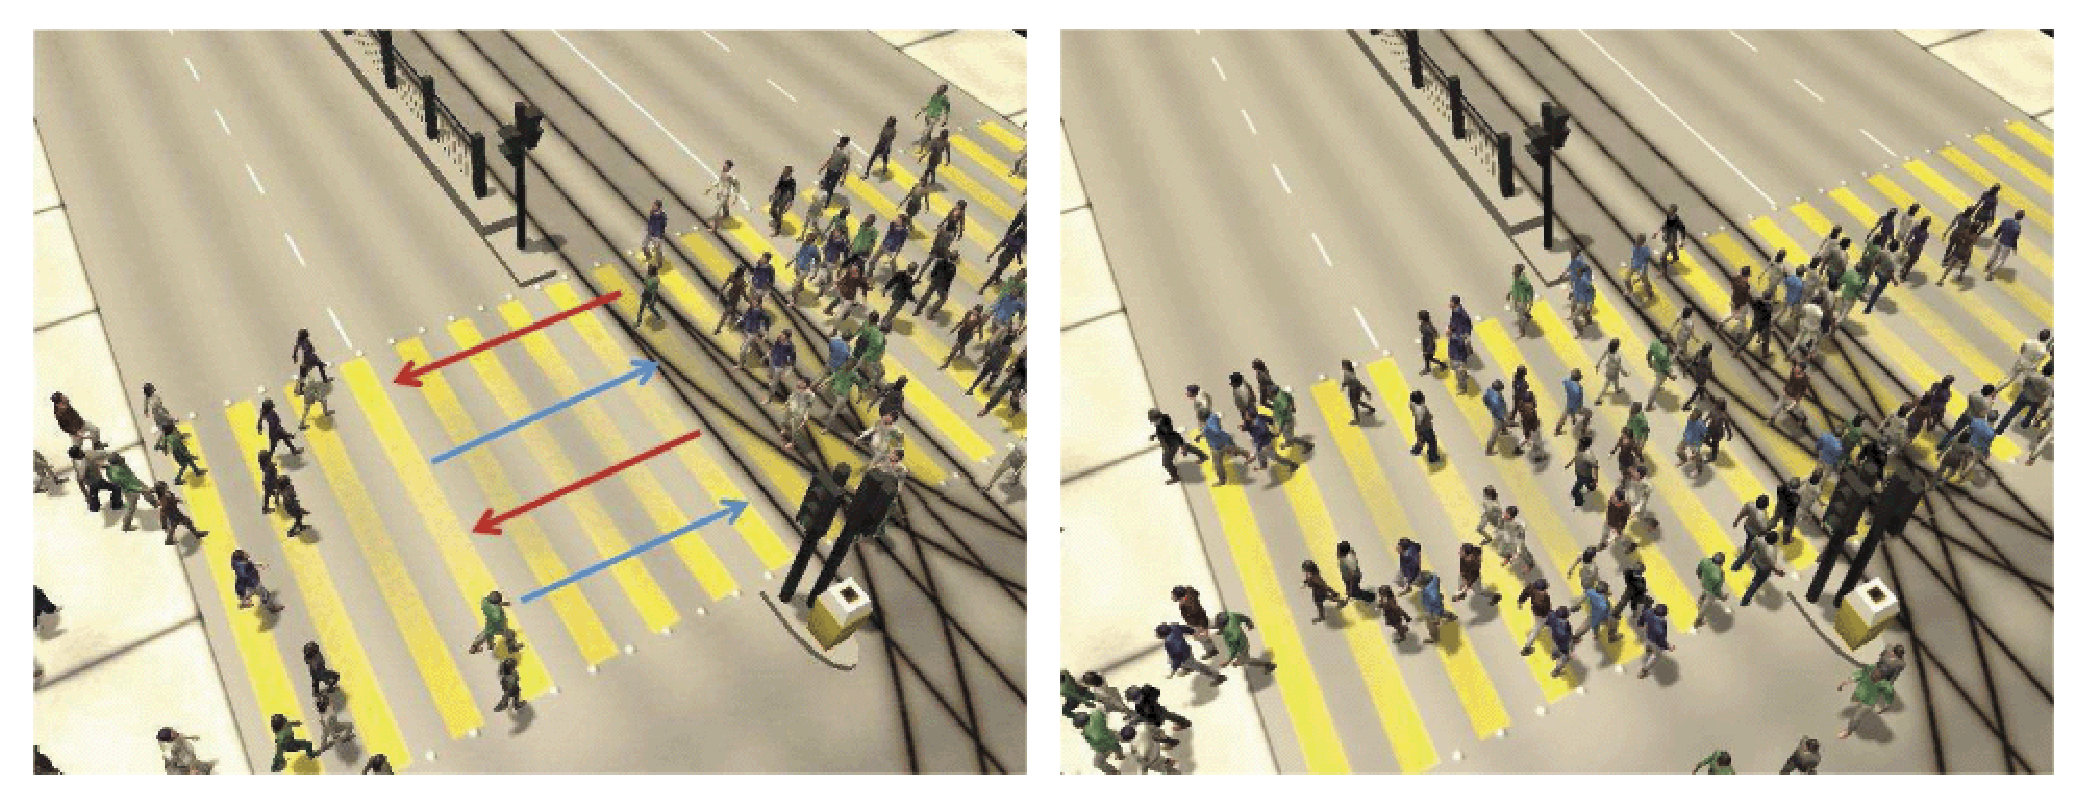
\includegraphics[scale=0.4]{navigation_fields.eps}
  \caption{Motion Planning for Crowd using Navigation Fields \citep{patil}}
  \label{fig:navigation}
\end{figure}

Extending the control vertically, in \citep{musse2} a hierarchical model for real time simulation of virtual human crowds is proposed allowing different control features at levels of crowd, groups or individuals. This is an example of hybrid approach where it is possible to increase the complexity of crowd-group-individual behaviours according to the problem to be simulated.

By means of these techniques, it was visually proven that very convincing and realistic results can be produced. Nevertheless, the identity and the decision capacity of each of the individuals is partially if not completely lost.

\section{Crowd Motion Simulation}

Purely simulation strategies, which is the case of this thesis, discard any pre-planned decision and the final result is entirely based on the global consequences of local interactions of members of the population. This is known as Agent-Based Model or Individual-Based Model. This will be detailed in Chapter \ref{chap:agent-based_model} and for further information check  \citep{red3D}.

The main idea this thesis is settled on is the simple principle stated by C. Reynolds, the pioneer of flocking behaviours, which claimed that very simple rules can arise emergent behaviours without involving any central coordination. Notice again the concept of emerge.

One of the earliest works  in group behaviours was Craig Reynolds' flocking algorithm which was a distributed behaviour model for flocks, herds and schools \citep{reynolds}. The individuals of his flocking system are called ``Boids'' and are subjected to three simple rules: cohesion, alignment and separation.

This classic research not only presents a flocking algorithm, but also marks a turning point proposing an individual virtual force model as the way to affect how each agent move. The approach presented in this thesis has adopted that model.

\begin{figure}[!htb]
  \centering
  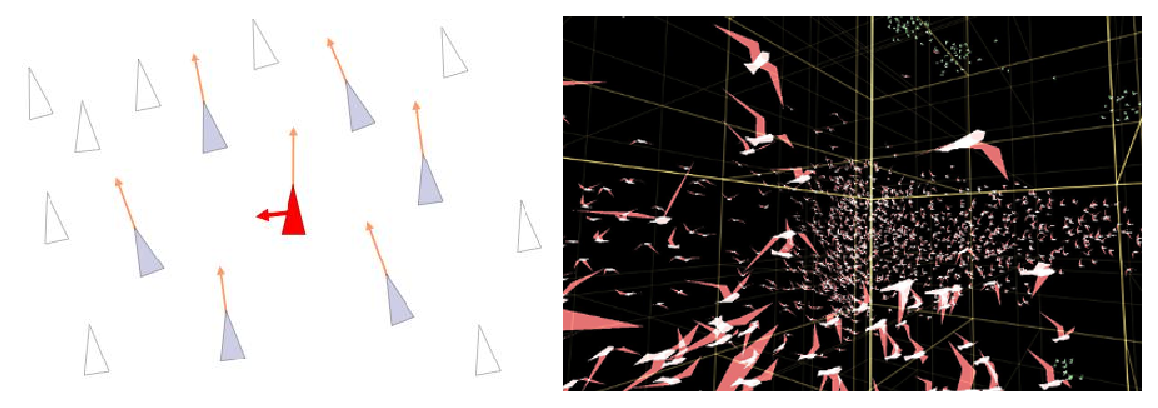
\includegraphics[scale=0.65]{reynolds_flocking.eps}
  \caption{Flocking System following the Virtual Force Model proposed by C. W. Reynolds \citep{reynolds}}
  \label{fig:massive}
\end{figure}

Starting from this robust and solid idea, tons of research paths can be taken in order to acquire and compare different approaches for crowd simulation. For instance, C. Wang \& T. Li suggest an evolving crowd motion simulation \citep{wang}. In that research, the use of genetic algorithms is proposed to generate optimal virtual forces according to the given environment and desired movement behaviour.

Although Craig Reynolds presents a base-approach which models very accurately the way crowds behave in the real world, the main disadvantage is that configuring the forces in order to generate desired motion behaviours remains empirical. And again, we are witnesses of a characteristic inherent to emergent behaviours.

\section{MASSIVE Software}

MASSIVE stands for Multiple Agent Simulation System in Virtual Environment and is a software developed by Stephen Regelous in Weta Digital, as a request from Peter Jackson to recreate those epic battle scenes that Tolkien described in the books of the Lord of the Rings. Massive has contributed to the creation of many awarding visual effects, particularly  the sequences; and due to this, it has been developed into a complete product and has been licensed by many other visual effects houses.

\begin{figure}[!htb]
  \centering
  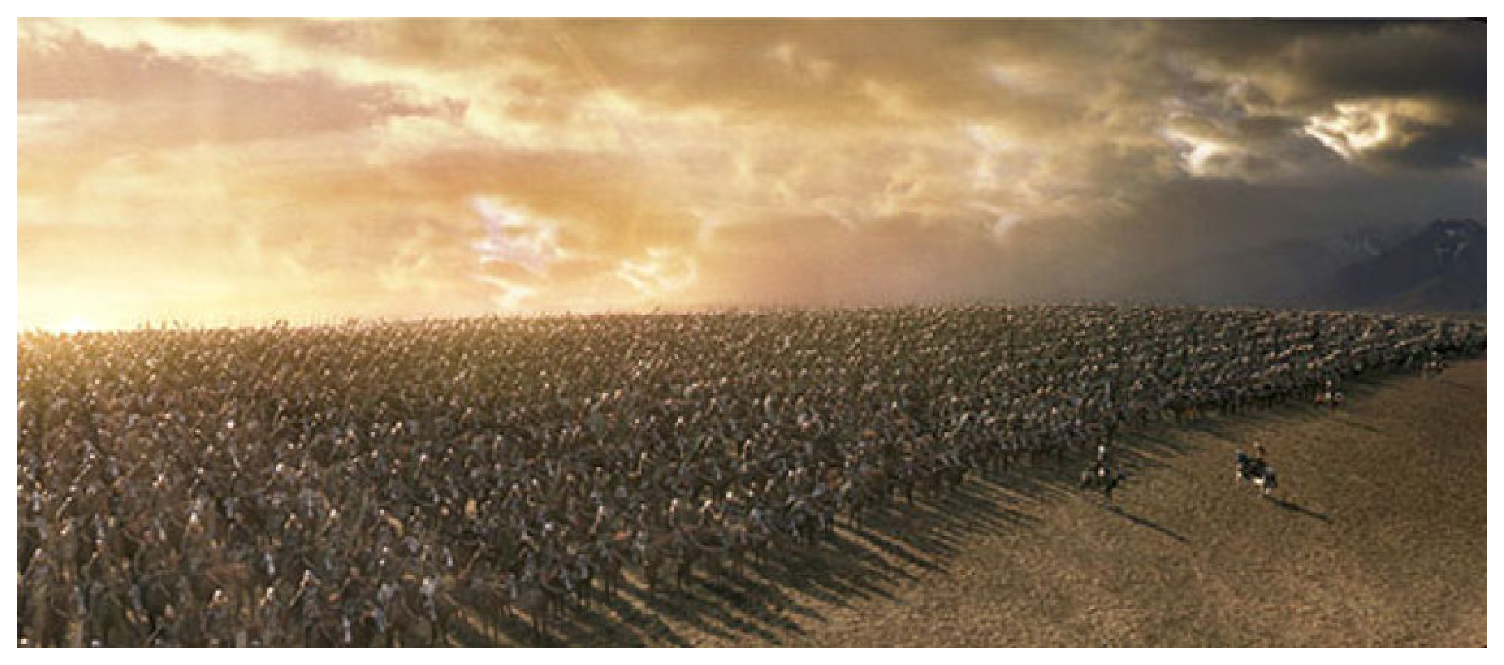
\includegraphics[scale=0.5]{rohan_army.eps}
  \caption{Award winning battle scene from 'The Lord of the Rings: Return of the King'}
  \label{fig:massive}
\end{figure}

Massive introduces a very interesting model approach which consists in treating each agent as a combination of a body and a brain. The body defines the physical characteristic of the agent and the brain is a fuzzy logic network which controls the actions of the agent such as following an arbitrary terrain, avoiding obstacles or interacting with other agents. This thesis has adopted this natural design combined with the flexibility that scripting languages provide.

Each action is associated to a pre-recorded animation, rather obtained from motion captured session or hand-animated, and will be blended between them in order to achieve the movement of the character. Apart from Artificial Intelligence features, it includes other abilities such as Rigid Body Dynamics (RBD), cloth simulation or GPU rendering. 



\ifx\isEmbedded\undefined
% References
\addcontentsline{toc}{chapter}{References}
\bibliographystyle{../ref/harvard}
\bibliography{../ref/master}
\pagebreak
\end{document}
\fi